\documentclass[aspectratio=43]{beamer}
\usetheme{Berlin}

\usepackage[english]{babel}
\usecolortheme{dolphin}
\usepackage{collargs}
\usepackage{tikz}
\usepackage{tikz-cd}
\usetikzlibrary{arrows.meta,calc,decorations.pathreplacing}

\usepackage{graphicx}
\usepackage{dirtree}
\usepackage{listings}
\usepackage[T1]{fontenc}
\usepackage{lmodern}
\usepackage[utf8]{inputenc}
\usepackage{caption}
\usepackage{bbding}
\usepackage{xurl}
\usepackage{scrextend}
\usepackage{minted}
\usepackage{appendixnumberbeamer}
\usepackage[backend=bibtex, style=numeric, maxcitenames=1, isbn=false, url=false, doi=false, eprint=false]{biblatex}

\addbibresource{../../doc/bibliography.bib}

\captionsetup{labelformat=empty}

\beamertemplatenavigationsymbolsempty
\defbeamertemplate*{title page}{customized}[1][]
{
\usebeamerfont{title}\inserttitle\par
\usebeamerfont{subtitle}\usebeamercolor[fg]{subtitle}\insertsubtitle\par
\bigskip
\usebeamerfont{author}\insertauthor\par
\usebeamerfont{institute}\insertinstitute\par
\usebeamerfont{date}\insertdate\par
\usebeamercolor[fg]{titlegraphic}\inserttitlegraphic
}

\hypersetup{unicode}
\hypersetup{breaklinks=true}

\title{LP $\Rightarrow$ CP 3D Printed Reflectarray}
\subtitle{Prepared for meeting on 10.22.2026}
\author{Havránek Kryštof}
\date{}
\institute{CTU, NTUST}
\setbeamertemplate{sidebar right}{}
\setbeamertemplate{footline}{%
\hfill\textbf{\insertframenumber{}/\inserttotalframenumber} \hspace{0.01cm} \vspace{0.1cm}}
\setbeamerfont{footnote}{size=\tiny}

\begin{document}

\begin{frame}[plain]
  \maketitle
\end{frame}

\clearpage
\setcounter{framenumber}{0}

% =====================================================================
\section{Introduction}
\begin{frame}[fragile]
  \frametitle{What We Are Trying To Do}
  \begin{itemize}
    \item Design a \textbf{reflectarray antenna} whose unit cell is
      \textbf{purely dielectric} (no metallisation of the elements).
      \begin{itemize}
        \item Only the ground plane is conductive.
        \item Elements additively manufactured (\textbf{FDM} / SLA).
      \end{itemize}
    \item Simultaneously achieve \textbf{beam focusing} \emph{and}
      \textbf{LP~$\Rightarrow$~CP polarization conversion} from a single
      linearly polarized feed.
    \item The cell must therefore control \textbf{two orthogonal reflection
        phases} independently.
    \item Target frequency: dictated purely by manufacturing technology -- resolution x print bed size.
  \end{itemize}
\end{frame}

% =====================================================================
\section{Physics}

\begin{frame}[fragile]
  \frametitle{Proposed Unit Cell Geometry}
  \begin{center}
    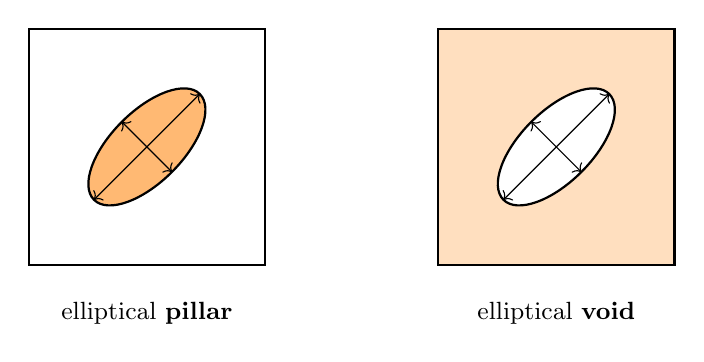
\begin{tikzpicture}[scale=1.0]
      % square half-side (tile)
      \def\H{1.5}

      % ---------- PILLAR (left) ----------
      \draw[thick] (-2.6-\H,-\H) rectangle (-2.6+\H,\H);
      \begin{scope}[shift={(-2.6,0)}, rotate=45]
        \filldraw[orange!55,draw=black,thick] (0,0) ellipse (0.95 and 0.45);
        \draw[<->,black] (-0.95,0) -- (0.95,0);
        \draw[<->,black] (0,-0.45) -- (0,0.45);
      \end{scope}
      \node[below] at (-2.6,-\H-0.35) {\small elliptical \textbf{pillar}};

      % ---------- VOID (right) ----------
      \fill[orange!25] (2.6-\H,-\H) rectangle (2.6+\H,\H);
      \draw[thick] (2.6-\H,-\H) rectangle (2.6+\H,\H);
      \begin{scope}[shift={(2.6,0)}, rotate=45]
        \filldraw[white,draw=black,thick] (0,0) ellipse (0.95 and 0.45);
        \draw[<->,black] (-0.95,0) -- (0.95,0);
        \draw[<->,black] (0,-0.45) -- (0,0.45);
      \end{scope}
      \node[below] at (2.6,-\H-0.35) {\small elliptical \textbf{void}};
    \end{tikzpicture}
  \end{center}
  \vspace{0.2cm}
  \begin{itemize}
    \item \textbf{Pillar} variant: better printability (no thin walls).
    \item \textbf{Void} variant: baseline solid dielectric, smoother phase
      response (backs away from resonance).
    \item In case of print issues $\Rightarrow$ rhombus, hexagon-esque structure, etc.
  \end{itemize}
\end{frame}


\begin{frame}[fragile]
  \frametitle{The Physics: Form Birefringence + Resonance}
  Two mechanisms work together:
  \begin{itemize}
    \item \textbf{Form birefringence} sets the \textbf{anisotropy}.
      \begin{itemize}
        \item Elliptical (not circular) cross-section.
        \item Sub-wavelength feature $\Rightarrow$ different effective
          permittivity along major vs.\ minor axis:
          $n_{\parallel} \neq n_{\perp}$.
      \end{itemize}
    \item \textbf{Reflection resonance} sets the \textbf{phase range}.
      \begin{itemize}
        \item UC acts as de-tuned resonator.
        \item Driving each axis through resonance swings the phase up to
          $360^\circ$.
      \end{itemize}
  \end{itemize}
\end{frame}

% =====================================================================
\begin{frame}[fragile]
  \frametitle{How the Two Mechanisms Couple}
  \begin{itemize}
    \item Because the two axes have \textbf{different effective permittivities},
      their resonances occur at \textbf{different pillar sizes} $a$.
    \item Form birefringence therefore \textbf{shifts the resonance location}
      between axes.
    \item The aspect ratio $a/b$ tunes how far apart the two resonances sit,
      and hence the achievable $90^\circ$ offset.
  \end{itemize}
  \begin{alertblock}{Design Tension}
    $\Delta\phi_x = 360^\circ$ wants a \emph{sharp} resonance;\\
    a stable $90^\circ$ offset to the other axis wants the two resonances
    \emph{close together}. These pull in opposite directions.
  \end{alertblock}
\end{frame}

% =====================================================================
\section{Unit Cell Design}

\begin{frame}[fragile]
  \frametitle{Unit Cell Geometry --- Parameters}
  \begin{center}
    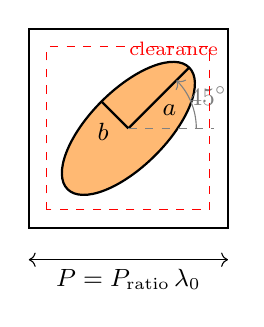
\begin{tikzpicture}[scale=1.15]
      % square footprint
      \draw[thick] (0,0) rectangle (2.2,2.2);
      % P_ratio: cell side
      \draw[<->] (0,-0.35) -- (2.2,-0.35);
      \node[below] at (1.1,-0.35) {\small $P = P_{\mathrm{ratio}}\,\lambda_0$};

      % cell centre
      \coordinate (c) at (1.1,1.1);

      % rotated ellipse
      \begin{scope}[rotate around={45:(c)}]
        \filldraw[orange!55,draw=black,thick] (c) ellipse (0.95 and 0.42);
      \end{scope}

      % a : semi-major axis
      \draw[-,thick] (c) -- ++(45:0.95) node[midway,above left,yshift=-10pt, xshift=10pt] {\small $a$};
      % b : semi-minor axis
      \draw[-,thick] (c) -- ++(135:0.42) node[midway,above right,xshift=-10pt, yshift=-13pt] {\small $b$};

      % rotation angle indicator
      \draw[dashed,gray] (c) -- ++(0:0.95);
      \draw[->,gray] ($(c)+(0:0.75)$) arc[start angle=0,end angle=45,radius=0.75];
      \node[gray] at ($(c)+(22:0.95)$) {\small $45^\circ$};

      % clearance
      \draw[dashed,red] (0.2,0.2) rectangle (2.0,2.0);
      \node[red,below] at (1.6,2.16) {\scriptsize clearance};
    \end{tikzpicture}
  \end{center}
  \vspace{0.1cm}
  \begin{itemize}
    \item $a$, $b$ --- semi-major/minor axes of the element, $\frac{a}{b} = $ \verb|ratio|.
    \item $P$ --- cell footprint, set by \verb|P_ratio|.
    \item Major axis rotated $45^\circ$ relative to the array axes.
      \begin{itemize}
        \item When illuminated by LP wave the incident wave can be seen as superposition of two LP waves aligned with principal axis.
      \end{itemize}
    \item Clearance dictated by manufacturing technology -- need to avoid thin walls, or bridging.
  \end{itemize}
\end{frame}

% =====================================================================
\begin{frame}[fragile]
  \frametitle{Unit Cell Design --- Prior Art}
  \begin{center}
    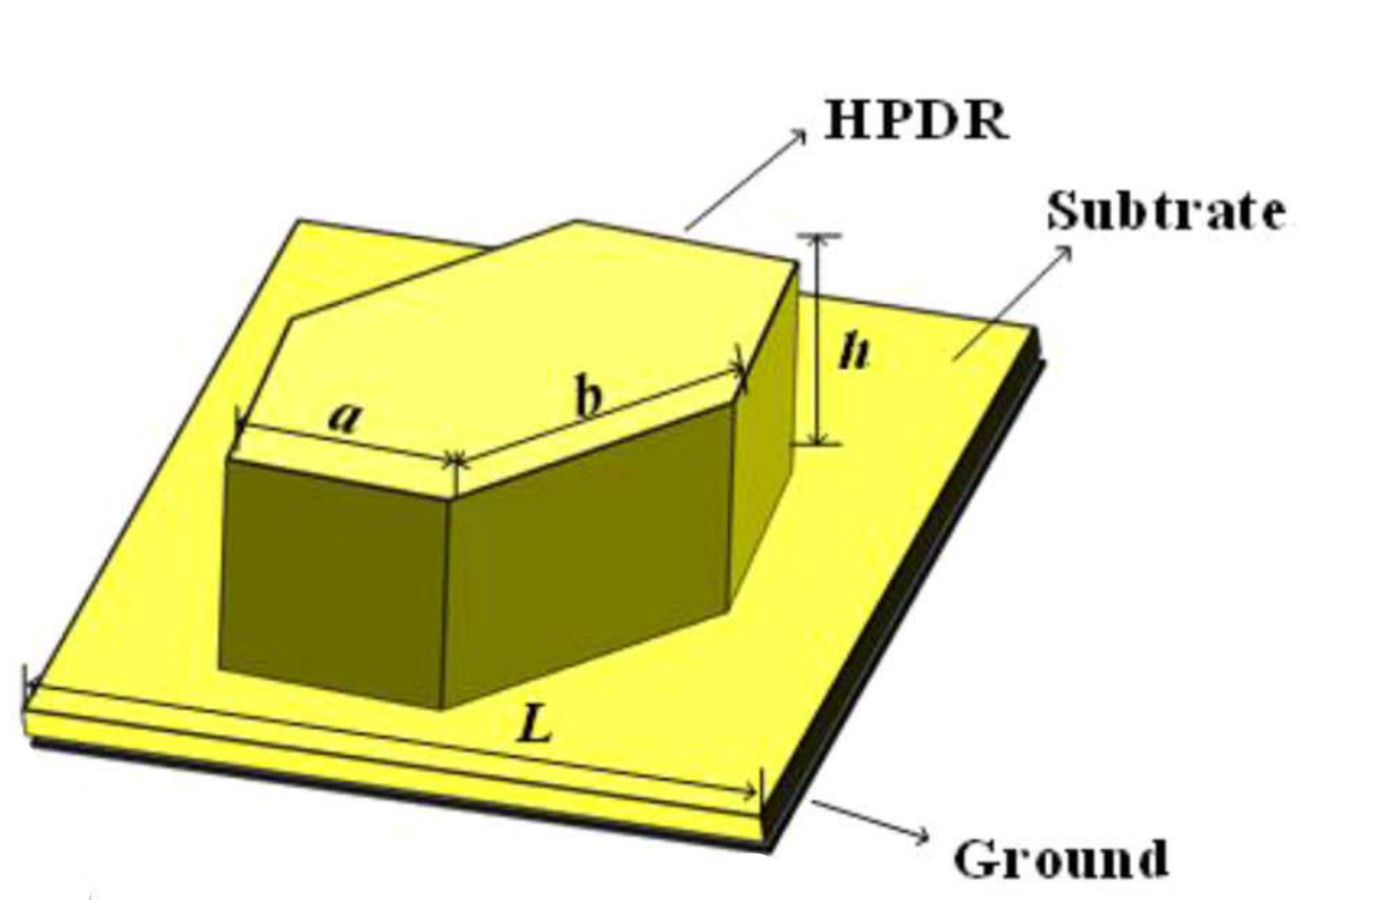
\includegraphics[width=0.4\textwidth]{./img/hao.jpg}
  \end{center}
  \begin{itemize}
    \item Hexagonal-prism dielectric resonator \footfullcite{Hao2020}
      \begin{itemize}
        \item Exhibits Form-Birefringence in $x$ and $y$ axis, profile is fixed.
        \item Roughly equal-amplitude $R_{xx}$ / $R_{xy}$ and a \textbf{constant $90^\circ$} phase difference gives LP--CP conversion.
        \item \textbf{Phase range from varying height}: $5.5 \to 23$~mm gives $> 360^\circ$; the $90^\circ$ offset stays constant with height.
        \item Multiple modes at higher heights with high bandwidth?
      \end{itemize}
  \end{itemize}
\end{frame}

\begin{frame}[fragile]
  \frametitle{Unit Cell Design --- Prior Art}
  \begin{center}
    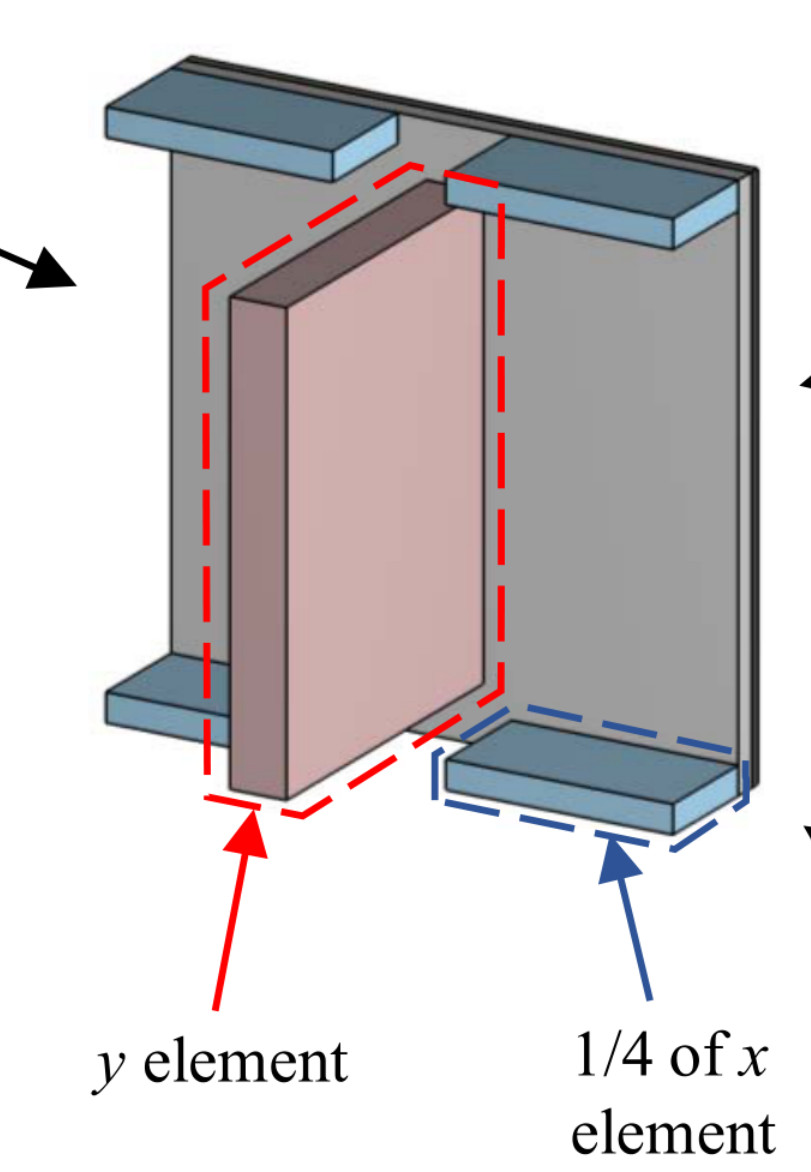
\includegraphics[width=0.2\textwidth]{./img/cheng.jpg}
  \end{center}
  \begin{itemize}
    \item Five  dielectric cuboids ($L\times W\times H$) in one cell \footfullcite{Cheng2022}.
      \begin{itemize}
        \item The $y$ element ($L_y, W_y, H_y$) reflects the $y$-polarized wave;
          the $x$ element (comprised of 4 smaller blocks) reflects the $x$-polarized wave.
        \item Phases tuned \emph{independently} by $H_x, H_y$,
          giving two orthogonal LP waves that recombine into a CP wave.
      \end{itemize}
  \end{itemize}
\end{frame}


% =====================================================================
\begin{frame}[fragile]
  \frametitle{How Our Cell Differs}
  \begin{itemize}
    \item Both prior designs achieve the per-axis phase by varying
      \textbf{height} (Hao) or by \textbf{two separate height-tuned blocks}
      (Cheng).
    \item \textbf{Our proposal:} a \textbf{single element of uniform height},
      where the two degrees of freedom come from \textbf{geometry changes in
        the $x$ and $y$ directions} rather than height.
      \begin{itemize}
        \item Uniform height $\Rightarrow$ flat, mechanically robust surface.
        \item No tall towers that block the wave reaching neighbouring cells -- important for phase wraps on some zone boundaries.
      \end{itemize}
    \item This variant does not appear to have been demonstrated before.
  \end{itemize}
\end{frame}

\begin{frame}[fragile]
  \frametitle{Challenges}
  \begin{itemize}
    \item \textbf{Existence of the unit cell}
      \begin{itemize}
        \item Can unit cell with large range phase range that maintains $\Delta \varphi = 90^\circ$ exists?
        \item At what frequencies are the properties reasonable?
      \end{itemize}
    \item \textbf{Measurement}
      \begin{itemize}
        \item Measuring permittivity of the material (most likely Zetamix 4.5 or 7.5)
        \item Verifying properties of the unit cell -- polarization, angle of incidence control.
          \begin{itemize}
            \item Free-space quasi-optical approach
            \item Parallel-plate waveguide -- requires smaller sample, less known method.
          \end{itemize}
      \end{itemize}
    \item \textbf{Manufacturing}
      \begin{itemize}
        \item Limited resolution of the printer -- nozzle at min 0.2~mm.
        \item Limited capabilities of the slicer -- some studies set infill to e.g. 90~\%, neglecting that for small features the slicer will print them solid.
      \end{itemize}
  \end{itemize}
\end{frame}



\section{feasibility Study}

% =====================================================================
\begin{frame}[fragile]
  \frametitle{Simulation Process --- Overview}
  \begin{enumerate}
    \item \textbf{Unit-cell model} in CST Microwave Studio
      (Floquet port, periodic boundaries).
    \item \textbf{Excitation:} TE$_{00}$ (x-pol) and TM$_{00}$ (y-pol) modes,
      normal incidence.
    \item Because the ellipse is rotated $45^\circ$, the x/y modes are not eigenpolarizations CST's output shows strong cross-coupling.
    \item Recover the principal-axis phases by rotating the
      $2\times2$ reflection matrix by $45^\circ$ in post-processing.
    \item Sweep geometry, extract phase range and inter-axis offset.
  \end{enumerate}
\end{frame}

% =====================================================================
\begin{frame}[fragile]
  \frametitle{Simulation Process --- The Chain}
  \begin{itemize}
    \item \textbf{CST}: parametric sweeps (ellipse size $a$, aspect ratio,
      permittivity, pillar height, cell size).
    \item \textbf{Export}: Touchstone \texttt{.s2p} per configuration $+$ with VBA macro.
    \item \textbf{MATLAB}: load all runs, rotate each $2\times2$ matrix to the
      eigenbasis, extract
      \begin{itemize}
        \item $|\phi_{\mathrm{major}} - \phi_{\mathrm{minor}}|$ (the $90^\circ$ offset),
        \item Find configuration with larger usable phase arc.
      \end{itemize}
    \item Usable arc is dictated by  $|S_{11}|$ and slope of phase change rate ($\leq 400^\circ/\mathrm{mm}$)
      \begin{itemize}
        \item Is ($\leq 400^\circ/\mathrm{mm}$) too conservative? maybe -- some studies use steeper slopes.
        \item Lower frequencies will fair much better -- UC is bigger, slope can be less steep.
      \end{itemize}

  \end{itemize}
\end{frame}

\begin{frame}[fragile]
  \frametitle{Simulation Results}
  \begin{itemize}
    \item Experimented mainly with pillar structure -- replicated Beccarias's study\footfullcite{Beccaria2025}
    \item For initial exploratory study \verb|ratio| is fixed to 1, $f_0 = 30~\mathrm{GHz}$
    \item Sampling in $a$ relatively low -- just 25 samples per range.
  \end{itemize}
  \begin{table}
    \caption{Phase range of cylindrical pillar}
    \begin{center}
      \begin{tabular}{| c | c | c || c |}
        \hline
        $\varepsilon_r$ & $P_\mathrm{ratio}$ & $H_\mathrm{pillar}$ (mm) & $\Delta \varphi_x$ (°) \\
        \hline
        4.5             & 0.4                & 5                        & 278.5                  \\
        5               & 0.4                & 5                        & 293.3                  \\
        5               & 0.5                & 5                        & 301.7                  \\
        6               & 0.5                & 4.2                      & 325.2                  \\


        \hline
      \end{tabular}
    \end{center}
  \end{table}
  \begin{itemize}
    \item for $P_\mathrm{ratio} = 0.5$ when $\varepsilon_r = 6$ there are resonance within feasible range of $a$.
    \item $P_\mathrm{ratio} = 0.3$ doesn't bring interesting results.
  \end{itemize}

\end{frame}

\begin{frame}[fragile]
  \frametitle{Simulation Results: Pillar, $P_\mathrm{ratio} = 0.4$, $\varepsilon_r  = 7$}
  \begin{center}
    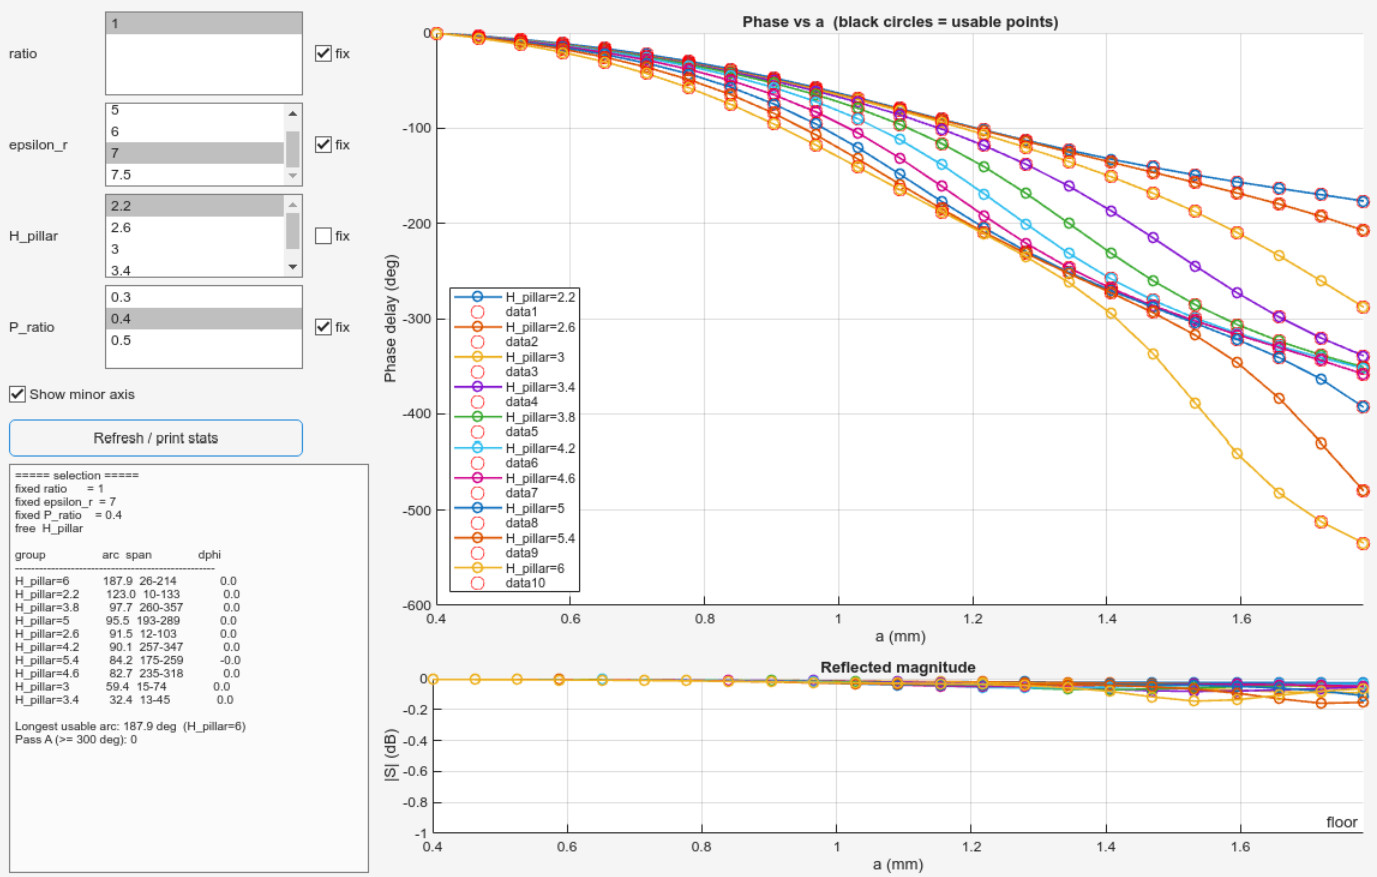
\includegraphics[width=\textwidth]{./img/er7_pillar.jpg}

  \end{center}
\end{frame}

\begin{frame}[fragile]
  \frametitle{Simulation Results: Cylindrical Void}
  \begin{itemize}
    \item Managed to run just $P_\mathrm{ratio} =0.4$ -- sweep already took many hours.
    \item Highest range of $270.8^\circ$ with $\varepsilon_r =6$ and $H_\mathrm{pillar} = 5$~mm
    \item Shape of the phase curves not too dissimilar, $S_{11}$ seems better?
    \item Problems with 3D printing -- pillars can use concentric infill.

  \end{itemize}

  \begin{minipage}{0.48\textwidth}
    \centering
    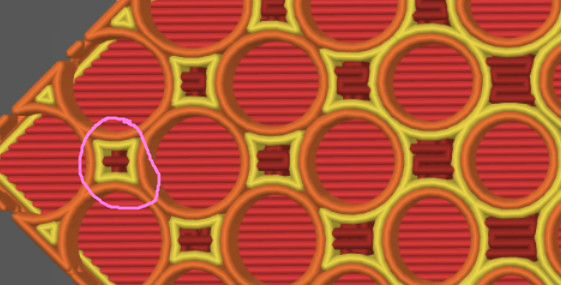
\includegraphics[width=.8\linewidth]{./img/void_recta.jpg}
  \end{minipage}\hfill
  \begin{minipage}{0.48\textwidth}
    \centering
    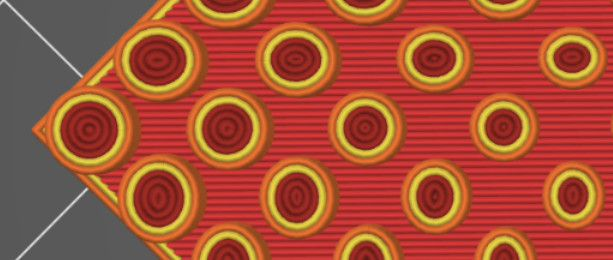
\includegraphics[width=.9\linewidth]{./img/pillar_concentric.jpg}
  \end{minipage}

\end{frame}

\begin{frame}[fragile]
  \frametitle{Simulation Results: Void, $P_\mathrm{ratio} = 0.4$, $\varepsilon_r  = 7$}
  \begin{center}
    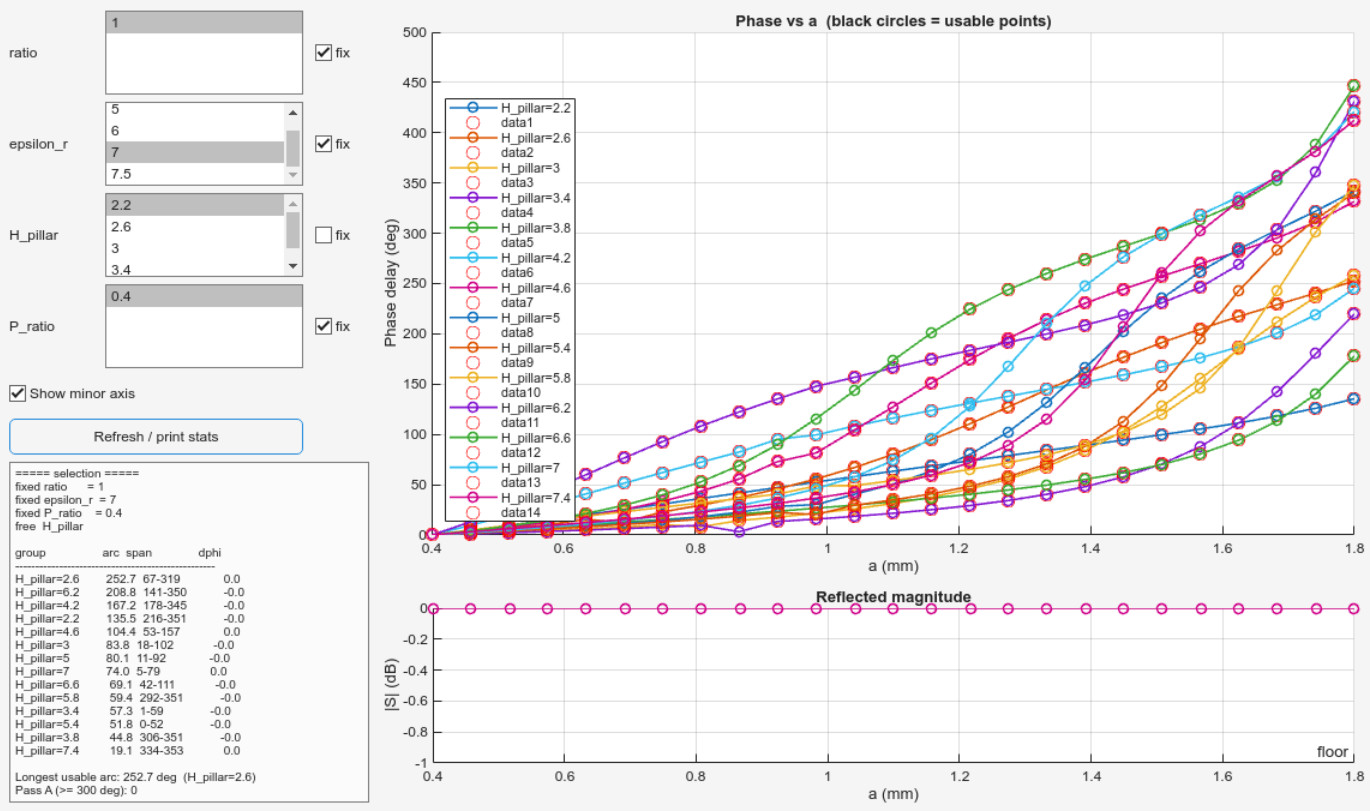
\includegraphics[width=\textwidth]{./img/er7_void.jpg}

  \end{center}
\end{frame}




% =====================================================================
\begin{frame}[fragile]
  \frametitle{Why Not Reaching 360$^\circ$ Hurts Us More}
  \begin{itemize}
    \item A \textbf{basic} reflectarray must hit any phase on the $0$--$360$ ring
      to compensate the feed-to-element path. $\sim 300^\circ$ is the accepted
      engineering threshold.
    \item Losing phase range raises a \textbf{phase error} at every element.
    \item In an \textbf{LP} array this error degrades \textbf{gain} and raises
      \textbf{sidelobes} -- bad, but tolerable.
  \end{itemize}
  \begin{alertblock}{It is worse for LP--CP}
    \begin{itemize}
      \item CP requires the two orthogonal components to stay at
        \textbf{equal amplitude and $90^\circ$ apart} \emph{at every element}.
      \item A missing phase range means the element cannot hit its required
        \emph{offset}, not merely its required focus phase.
      \item Polarization-purity loss, not just a focusing loss.
    \end{itemize}
  \end{alertblock}
\end{frame}



% =====================================================================
\begin{frame}[fragile]
  \frametitle{Escalation Path if the Two Degrees of Freedom Fall Short}
  \begin{itemize}
    \item If height + uniform geometry cannot deliver the range \emph{and}
      a stable $90^\circ$ offset:
      \begin{itemize}
        \item add a \textbf{third degree of freedom} to the cell, or
        \item adopt \textbf{multiple resonances}
      \end{itemize}
    \item \textbf{More resonances:}
      \begin{itemize}
        \item Each added resonance sharpens the phase slope, trading \textbf{bandwidth} for range.
        \item Limited by printer resolution.
      \end{itemize}
    \item \textbf{3 parameters:} (\verb|a|, \verb|ratio|, \verb|H_pillar|) design is more complicated $\Rightarrow$ MLP based surrogate model + NGSA-II to find optimal solutions if the behavior isn't nice.
  \end{itemize}
\end{frame}

% footfullcite

\end{document}
